\chapter{矢量分析}
\section{nabla算符$\nabla$;梯度;散度;旋度;张量积}
这一章与矢量和微积分有关,以后讲电动力学的时候会用到。你可以想一想电磁学中的例子,还可以用软件画一些矢量场试试看。

首先要讲一个符号$\nabla$读作nabla。(也有人会读成del,还有些地方叫作哈密顿算符,但是这样会跟量子力学中的哈密顿算符搞混)它既是矢量,又是算符。在三维直角坐标系中,$\nabla=(\ppx,\ppy,\ppz)$。简单起见,接下来遇到的大多是二维的情况。

$\nabla$可以作用到标量或者矢量上面。把它作用到标量$f$上面,会变成一个矢量:$\nabla f=(\frac{\partial f}{\partial x},\frac{\partial f}{\partial y},\frac{\partial f}{\partial z})$,称为$f$的梯度。

如果$f$是$x,y,z$的函数,相当于在空间中的每个点都有一个$f$的值,我们说$f$是一个标量场。同样,空间中的每个点都有一个矢量$\nabla f$,我们说$\nabla f$是一个矢量场。

举个栗子:$f=x^2+y$,$\nabla f=(2x,1,0)$,如图\ref{fig-vec-grad},越白的地方$f$越大。
\begin{figure}[htb]
\centering
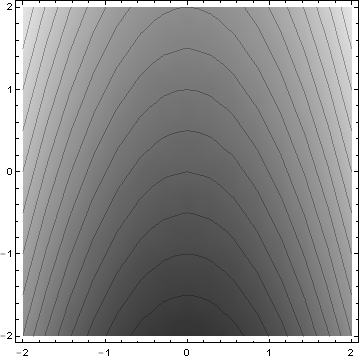
\includegraphics[scale=0.5]{fig/vec-grad.png}
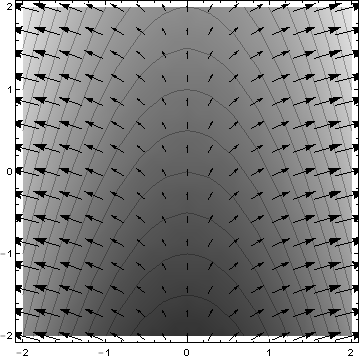
\includegraphics[scale=0.5]{fig/vec-grad-2.png}
\caption{沿着箭头爬上去}
\label{fig-vec-grad}
\end{figure}

$\nabla f$表示$f$变化的快慢和方向。比如$f$是电势,$-\nabla f$就是电场。

如果把$\nabla$作用到矢量上面,一般有三种方法:点积,叉积,张量积。$\nabla$与矢量$\mathbf{A}$点积,会变成一个标量:$\nabla \cdot \mathbf{A}=\frac{\partial A_x}{\partial x}+\frac{\partial A_y}{\partial y}+\frac{\partial A_z}{\partial z}$,称为$\mathbf{A}$的散度。

举个栗子:$\mathbf{A}=(1-x^2,y,0)$,$\nabla \cdot \mathbf{A}=1-2x$,如图\ref{fig-vec-div},越白的地方$\nabla \cdot \mathbf{A}$越大。
\begin{figure}[htb]
\centering
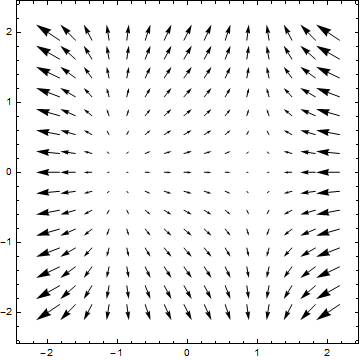
\includegraphics[scale=0.5]{fig/vec-div.png}
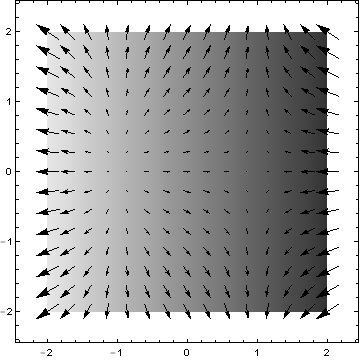
\includegraphics[scale=0.5]{fig/vec-div-2.png}
\caption{箭头出来了又进去了}
\label{fig-vec-div}
\end{figure}

$\nabla \cdot \mathbf{A}$表示$\mathbf{A}$在某个点上变多的程度,负数则表示变少。图\ref{fig-vec-div}的左边比较白,$\nabla \cdot \mathbf{A}>0$,可以看到从某个点出来的箭头比进去的大;右边比较黑,$\nabla \cdot \mathbf{A}<0$,进去的箭头比出来的大。

比如正的点电荷上面的$\nabla \cdot \mathbf{E}>0$,没有电荷的地方$\nabla \cdot \mathbf{E}=0$。如果一条河里的水流速度为$\mathbf{v}$,即使我们不知道水是怎么流的,但是任何一个点进去和出来的水肯定一样多,所以$\nabla \cdot \mathbf{v}=0$。

$\nabla$与矢量$\mathbf{A}$叉积,仍然是一个矢量(背一遍叉积的公式):$\nabla \times \mathbf{A}=(\frac{\partial A_z}{\partial y}-\frac{\partial A_y}{\partial z},\frac{\partial A_x}{\partial z}-\frac{\partial A_z}{\partial x},\frac{\partial A_y}{\partial x}-\frac{\partial A_x}{\partial y})$,称为$\mathbf{A}$的旋度。

举个栗子:$\mathbf{A}=(-\frac{y}{x^2+y^2+1},\frac{x}{x^2+y^2+1},0)$,$\nabla \times \mathbf{A}=(0,0,\frac{2}{(x^2+y^2+1)^2})$。因为$\mathbf{A}$只有$x,y$分量,所以$\nabla \times \mathbf{A}$只有$z$分量。如图\ref{fig-vec-curl},越白的地方$(\nabla \cdot \mathbf{A})_z$越大。
\begin{figure}[htb]
\centering
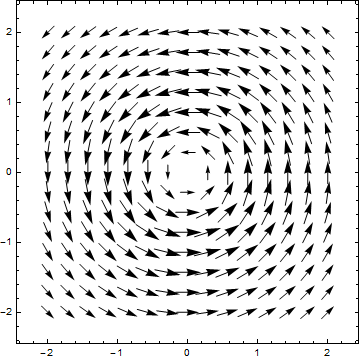
\includegraphics[scale=0.5]{fig/vec-curl.png}
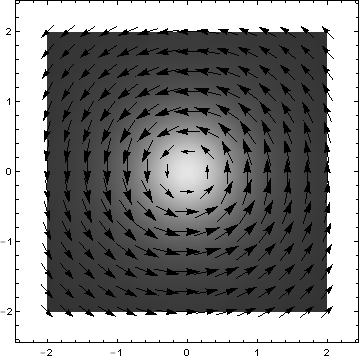
\includegraphics[scale=0.5]{fig/vec-curl-2.png}
\caption{高速旋转!面对疾风吧!!!!}
\label{fig-vec-curl}
\end{figure}

$\nabla \times \mathbf{A}$表示$\mathbf{A}$在某个点上旋转的程度,以及旋转的方向(用右手螺旋表示)。图\ref{fig-vec-curl}中的箭头全都在逆时针转,所以$\nabla \times \mathbf{A}$指向$+z$方向。比如电流$I$周围会形成一圈圈磁场,$\nabla \times \mathbf{B}$指向电流方向。

如果$\mathbf{A}$是匀强场,那么$\nabla \cdot \mathbf{A}=0$,$\nabla \times \mathbf{A}=\mathbf{0}$。

如果知道(空间中每个点的)$\nabla f$,通过积分就能确定$f$,最多相差一个积分常量。知道$\nabla \cdot \mathbf{A}$和$\nabla \times \mathbf{A}$,通过更复杂的积分也能确定$\mathbf{A}$,最多相差一个常矢量。

最后是$\nabla$与$\mathbf{A}$的张量积,一般写成$\nabla \mathbf{A}$,中间没有$\cdot$也没有$\times$。(虽然有些人会用各种奇怪的写法)它一般出现在运算的中间过程,至于物理意义就很难讲。它是一个$3 \times 3$的张量:
\begin{equation}
\nabla \mathbf{A}=\partial_i A_j=\begin{bmatrix}
\frac{\partial A_x}{\partial x} & \frac{\partial A_y}{\partial x} & \frac{\partial A_z}{\partial x} \\
\frac{\partial A_x}{\partial y} & \frac{\partial A_y}{\partial y} & \frac{\partial A_z}{\partial y} \\
\frac{\partial A_x}{\partial z} & \frac{\partial A_y}{\partial z} & \frac{\partial A_z}{\partial z}
\end{bmatrix}
\end{equation}

还要注意,在不同的坐标系中,$\nabla$的分量是不同的,不一定只有偏导数。简单起见,接下来遇到的都是直角坐标系。
\section{高斯定理;斯托克斯定理}
在三维空间中随便画一个闭合曲面$S$,可以计算矢量场$\mathbf{A}$在$S$上的通量$\Phi=\oint_S \mathbf{A} \cdot \opd \mathbf{S}$。

($\oint_S$表示对$S$上的每个小面元进行积分,圆圈表示闭合曲面,这只是书写的一些习惯。有些地方会写成$\oiint$,表示小面元是二维的。矢量$\opd \mathbf{S}$表示一个有方向的小面元,它的大小是小面元的面积,方向垂直于小面元向外)

把$S$里面的区域记为$V$,计算$\int_V \nabla \cdot \mathbf{A} \opd V$。既然$\nabla \cdot \mathbf{A}$表示$\mathbf{A}$在某个点上变多了多少,把它对$V$积分就是$\mathbf{A}$在$S$里面总共多了多少。这些多出来的$\mathbf{A}$会从$S$上出去,就是$\Phi$。这个公式称为高斯定理:
\begin{equation*}
\oint_S \mathbf{A} \cdot \opd \mathbf{S}=\int_V \nabla \cdot \mathbf{A} \opd V
\end{equation*}

举个栗子:如图\ref{fig-gauss-flux},$\mathbf{A}=(1-x^2,y,0)$,画一个三角形$\triangle ABC$,$A(0,0,0),B(1,0,0),C(0,1,0)$。验证一下高斯定理:

(简单起见,我们把三维问题变成二维问题,现在$S$是三角形的边,$V$是三角形里面的面积)
\begin{figure}[htb]
\centering
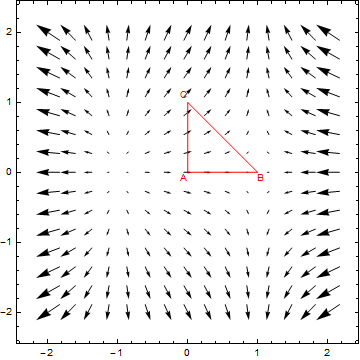
\includegraphics[scale=0.5]{fig/gauss-flux.png}
\caption{验证高斯定理}
\label{fig-gauss-flux}
\end{figure}
\begin{align*}
\nabla \cdot \mathbf{A}&=1-2 x \\
\int_V \nabla \cdot \mathbf{A} \opd V&=\int_{x=0}^1 \int_{y=0}^{1-x} (1-2 x) \opd x \opd y
\internote{(对面积积分可以对$x$和$y$分别积分。这里$y$的积分上限与$x$有关,所以要先对$y$积分,再对$x$积分)}
&=\int_0^1 \left( \int_0^{1-x} (1-2 x) \opd y \right) \opd x \\
&=\int_0^1 (1-x)(1-2 x) \opd x \\
&=\frac{1}{6}
\end{align*}

$\oint_S \mathbf{A} \cdot \opd \mathbf{S}$要在三条边上分开算。$AB$边上的$\mathbf{A}$平行于$AB$边,通量$\oint_{AB} \mathbf{A} \cdot \opd \mathbf{S}$显然是0。

$AC$边的单位法向量$\mathbf{n}_{AC}=(-1,0)$(注意要向外),$\mathbf{A} \cdot \mathbf{n}_{BC}|_{x=0}=-1$。$AC$边平行于$y$轴,$\opd \mathbf{S}$的大小就是$\opd y$。$\oint_{AC} \mathbf{A} \cdot \opd \mathbf{S}=\int_0^1 (-1) \opd y=-1$。

$BC$边是斜着的,所以会复杂一些。我们可以把它\emph{参数化}:定义一个参数$t$,它既表示$x$的变化,又表示$y$的变化。令$0<t<1$,$x=t$,$y=1-t$,$\opd S=\sqrt{(\opd x)^2+(\opd y)^2}=\sqrt{2} \opd t$。

$BC$边的单位法向量$\mathbf{n}_{BC}=(\frac{\sqrt{2}}{2},\frac{\sqrt{2}}{2})$,$\mathbf{A} \cdot \mathbf{n}_{BC}=\frac{\sqrt{2}}{2}(1-x^2+y)=\frac{\sqrt{2}}{2}(-t^2-t+2)$,$\oint_{BC} \mathbf{A} \cdot \opd \mathbf{S}=\int_0^1 \frac{\sqrt{2}}{2}(-t^2-t+2) \cdot \sqrt{2} \opd t=\frac{7}{6}$。

三条边上的通量加起来刚好是$\frac{1}{6}$,与散度的积分相等,跟高斯定理说的一样。

在三维空间中随便画一条闭合曲线$L$,还可以计算$\mathbf{A}$在$L$上的环量$C=\oint_L \mathbf{A} \cdot \opd \mathbf{L}$。

($\opd \mathbf{L}$沿着$L$的右手螺旋方向,左边是$L$的里面。里面和外面的严格定义很复杂,这里我们先用肉眼判断)

把$L$里面的区域记为$S$,计算$\int_S (\nabla \times \mathbf{A}) \cdot \opd \mathbf{S}$。如图\ref{fig-stokes-prove},每个$(\nabla \times \mathbf{A}) \cdot \opd \mathbf{S}$都表示一块小面元上$\mathbf{A}$的旋转程度,相邻两块小面元的公共边上$\mathbf{A}$会抵消,剩下最外面一圈就是$C$。这个公式称为斯托克斯定理:
\begin{equation*}
\oint_L \mathbf{A} \cdot \opd \mathbf{L}=\int_S (\nabla \times \mathbf{A}) \cdot \opd \mathbf{S}
\end{equation*}
\begin{figure}[htb]
\centering
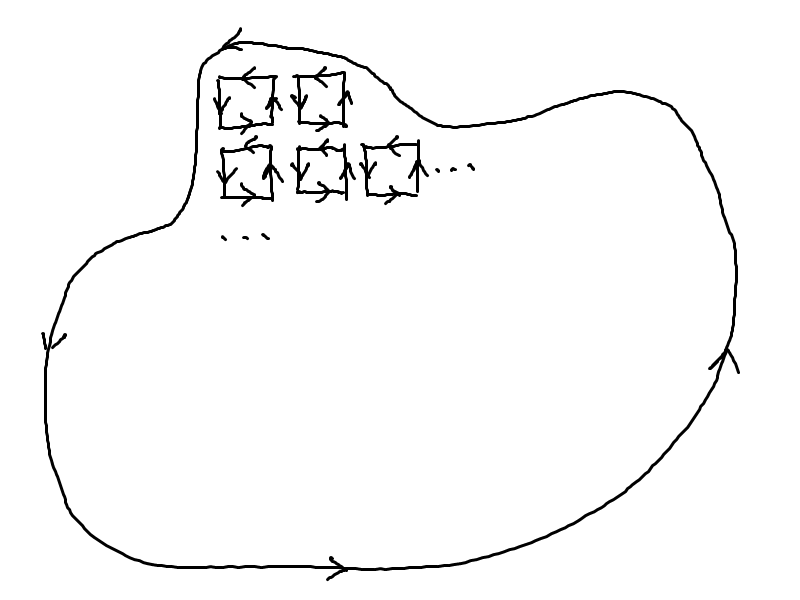
\includegraphics[scale=0.5]{fig/stokes-prove.png}
\caption{大家一起高速旋转}
\label{fig-stokes-prove}
\end{figure}

高斯定理和斯托克斯定理在二维情况下也成立,一维情况就是微积分中的牛顿-莱布尼兹定理:$F(b)-F(a)=\int_a^b F'(x) \opd x$。它们都把区域的边界和内部联系了起来。
\section{克罗内克张量$\delta_{i j}$;列维-奇维塔张量$\epsilon_{i j k}$;一些矢量公式}
方便起见,这一节用$1,2,3$表示$x,y,z$坐标,$\partial_i$表示$\frac{\partial}{\partial i}$。在三维直角坐标系中,$1 \le i,j \le 3$,$\mathbf{A}$就是$A_i$,$\nabla$就是$\partial_i$。

矢量$A_i$是有一个下标的量,张量则是有很多下标的量。矢量也是一种张量,前面的张量积$\nabla \mathbf{A}$则是有两个下标的张量。接下来我们用张量来表示一些矢量运算的公式,还会发现前面说的爱因斯坦求和约定非常方便。

(其实张量必须满足一些变换的规律,这里先不讲了。这里也不区分自由指标和哑指标)

矢量的点积$\mathbf{A} \cdot \mathbf{B}=\sum_{i=1}^3 A_i B_i$。按照爱因斯坦求和约定,下标相同就表示求和,求和号可以不写。也就是说,$\mathbf{A} \cdot \mathbf{B}=A_i B_i$。这样求和一次,式子中的下标就会减少两个,称为下标缩并。

克罗内克张量$\delta_{i j}=\begin{cases} 1, &i=j \\ 0, &i \neq j \end{cases}$。在三维情况下,$\delta_{i j}=\begin{bmatrix}
1 & 0 & 0 \\
0 & 1 & 0 \\
0 & 0 & 1
\end{bmatrix}$。如果把$\delta_{i j}$与$A_j$缩并,$\delta_{i j} A_j=A_i$,相当于给$A$换一个下标。

接下来讲一个复杂一些的张量:列维-奇维塔张量$\epsilon_{i j k}$,又叫排序张量。如果$ijk$分别是$123$,$231$或者$312$,那么$\epsilon_{i j k}=1$;如果$ijk$分别是$321$,$213$或者$132$,那么$\epsilon_{i j k}=-1$;否则$ijk$中至少有两个相同,$\epsilon_{i j k}=0$。它的分量形式这里就不写了,因为我懒。

矢量的叉积$\mathbf{A} \times \mathbf{B}=\epsilon_{i j k} A_j B_k$。它的左边是矢量,右边有一个自由指标$i$没有被求和,所以也是矢量。任何公式两边的自由指标必须是相同的(左边的矢量可以脑补下标$i$),而被求和的指标(哑指标,这里是$j,k$)可以不同。通过枚举可以发现:
\begin{align*}
(\mathbf{A} \times \mathbf{B})_1&=A_2 B_3-A_3 B_2 \\
(\mathbf{A} \times \mathbf{B})_2&=A_3 B_1-A_1 B_3 \\
(\mathbf{A} \times \mathbf{B})_3&=A_1 B_2-A_2 B_1
\end{align*}

容易发现,$\delta_{i j}=\delta_{j i}$,$\epsilon_{i j k}=\epsilon_{j k i}=-\epsilon_{j i k}$。还有一个公式:$\epsilon_{i j k} \epsilon_{k l m}=\delta_{i l} \delta_{j m}-\delta_{i m} \delta_{j l}$。这个公式也可以通过枚举来证明(虽然很麻烦):两边各有四个自由指标$i,j,l,m$,分别代进去$1,2,3$,共有81种情况,然后会发现它确实是对的。

接下来可以推导更复杂的公式:$(\mathbf{A} \times \mathbf{B}) \times \mathbf{C}=(\mathbf{A} \cdot \mathbf{C})\mathbf{B}-(\mathbf{B} \cdot \mathbf{C})\mathbf{A}$。
\begin{align*}
(\mathbf{A} \times \mathbf{B}) \times \mathbf{C}&=\epsilon_{i j k} (\epsilon_{j l m} A_l B_m) C_k \\
&=\epsilon_{i j k} \epsilon_{j l m} A_l B_m C_k
\internote{($\delta_{i j},\epsilon_{i j k},A_i$的指标缩并满足交换律和结合律)}
&=\epsilon_{k i j} \epsilon_{j l m} A_l B_m C_k \\
&=(\delta_{k l} \delta_{i m}-\delta_{k m} \delta_{i l}) A_l B_m C_k \\
&=\delta_{k l} \delta_{i m} A_l B_m C_k-\delta_{k m} \delta_{i l} A_l B_m C_k \\
&=A_k B_i C_k-A_i B_k C_k \\
&=(\mathbf{A} \cdot \mathbf{C})\mathbf{B}-(\mathbf{B} \cdot \mathbf{C})\mathbf{A}
\end{align*}

可以看出,如果在$(\mathbf{A} \times \mathbf{B}) \times \mathbf{C}$中交换$\mathbf{A}$和$\mathbf{B}$,结果会变成相反数。但是如果交换$\mathbf{A}$和$\mathbf{C}$,结果会完全不一样。

【练习】证明$\mathbf{A} \times (\mathbf{B} \times \mathbf{C})=(\mathbf{A} \cdot \mathbf{C})\mathbf{B}-(\mathbf{A} \cdot \mathbf{B})\mathbf{C}$。

把这个式子中的$\mathbf{A}$和$\mathbf{B}$换成$\nabla$,$\mathbf{C}$换成$\mathbf{A}$,还可以证明$\nabla \times (\nabla \times \mathbf{A})=\nabla(\nabla \cdot \mathbf{A})-(\nabla \cdot \nabla) \mathbf{A}$。

$(\nabla \cdot \nabla)$可以写成$\nabla^2$,称为拉普拉斯算符。在三维直角坐标系里,它就是$\ppxn{2}+\ppyn{2}+\ppzn{2}$。它没有下标,$\nabla^2 f$仍然是标量,$\nabla^2 \mathbf{A}$仍然是矢量。

但是要注意,$\partial_i$与$A_i$不满足交换律,因为$\partial_i$是对右边的东西求导,而$\partial_i$与$\partial_j,\delta_{i j},\epsilon_{i j k}$仍然满足交换律。比如要证明$\nabla \cdot (\mathbf{A} \times \mathbf{B})=\mathbf{B} \cdot (\nabla \times \mathbf{A})-\mathbf{A} \cdot (\nabla \times \mathbf{B})$:
\begin{align*}
\nabla \cdot (\mathbf{A} \times \mathbf{B})&=\partial_i (\epsilon_{i j k} A_j B_k) \\
&=\epsilon_{i j k} \partial_i(A_j B_k) \\
&=\epsilon_{i j k} (B_k \partial_i A_j+A_j \partial_i B_k) \\
&=B_k \epsilon_{k i j} \partial_i A_j+A_j \epsilon_{j k i} \partial_i B_k \\
&=B_k \epsilon_{k i j} \partial_i A_j-A_j \epsilon_{j i k} \partial_i B_k \\
&=\mathbf{B} \cdot (\nabla \times \mathbf{A})-\mathbf{A} \cdot (\nabla \times \mathbf{B})
\end{align*}

矢量分析当中常用的公式就是这么多,以后用到的时候可以翻回来看看。
